
\documentclass[12pt,journal,compsoc]{IEEEtran}


% *** CITATION PACKAGES ***
%
\ifCLASSOPTIONcompsoc
  % IEEE Computer Society needs nocompress option
  % requires cite.sty v4.0 or later (November 2003)
  \usepackage[nocompress]{cite}
\else
  % normal IEEE
  \usepackage{cite}
\fi
% cite.sty was written by Donald Arseneau
% V1.6 and later of IEEEtran pre-defines the format of the cite.sty package
% \cite{} output to follow that of IEEE. Loading the cite package will
% result in citation numbers being automatically sorted and properly
% "compressed/ranged". e.g., [1], [9], [2], [7], [5], [6] without using
% cite.sty will become [1], [2], [5]--[7], [9] using cite.sty. cite.sty's
% \cite will automatically add leading space, if needed. Use cite.sty's
% noadjust option (cite.sty V3.8 and later) if you want to turn this off.
% cite.sty is already installed on most LaTeX systems. Be sure and use
% version 4.0 (2003-05-27) and later if using hyperref.sty. cite.sty does
% not currently provide for hyperlinked citations.
% The latest version can be obtained at:
% http://www.ctan.org/tex-archive/macros/latex/contrib/cite/
% The documentation is contained in the cite.sty file itself.
%
% Note that some packages require special options to format as the Computer
% Society requires. In particular, Computer Society  papers do not use
% compressed citation ranges as is done in typical IEEE papers
% (e.g., [1]-[4]). Instead, they list every citation separately in order
% (e.g., [1], [2], [3], [4]). To get the latter we need to load the cite
% package with the nocompress option which is supported by cite.sty v4.0
% and later. Note also the use of a CLASSOPTION conditional provided by
% IEEEtran.cls V1.7 and later.





% *** GRAPHICS RELATED PACKAGES ***
%
\ifCLASSINFOpdf
  \usepackage[pdftex]{graphicx}
  % declare the path(s) where your graphic files are
  \graphicspath{{/beamer/}{../beamer/img/}}
  % and their extensions so you won't have to specify these with
  % every instance of \includegraphics
  \DeclareGraphicsExtensions{.pdf,.jpeg,.png}
  
  \usepackage{color}
  \usepackage{tikz}
\usetikzlibrary{decorations.markings}

\pgfdeclarelayer{edgelayer}
\pgfdeclarelayer{nodelayer}
\pgfsetlayers{edgelayer,nodelayer,main}

\tikzstyle{none}=[inner sep=0pt]
\definecolor{hexcolor0x0074ff}{rgb}{0.000,0.455,1.000}
\definecolor{hexcolor0xff2615}{rgb}{1.000,0.149,0.082}

\definecolor{myblack}{rgb}{0.000,0.000,0.000}
\definecolor{mywhite}{rgb}{1.000,1.000,1.000}

\tikzstyle{setA}=[circle,fill=hexcolor0x0074ff,draw=myblack]
\tikzstyle{setB}=[circle,fill=hexcolor0xff2615,draw=myblack]
\tikzstyle{node}=[circle,fill=mywhite,draw=myblack,scale=.1]
\else
  % or other class option (dvipsone, dvipdf, if not using dvips). graphicx
  % will default to the driver specified in the system graphics.cfg if no
  % driver is specified.
  \usepackage[dvips]{graphicx}
  % declare the path(s) where your graphic files are
  % \graphicspath{{../eps/}}
  % and their extensions so you won't have to specify these with
  % every instance of \includegraphics
  % \DeclareGraphicsExtensions{.eps}
\fi
% graphicx was written by David Carlisle and Sebastian Rahtz. It is
% required if you want graphics, photos, etc. graphicx.sty is already
% installed on most LaTeX systems. The latest version and documentation can
% be obtained at: 
% http://www.ctan.org/tex-archive/macros/latex/required/graphics/
% Another good source of documentation is "Using Imported Graphics in
% LaTeX2e" by Keith Reckdahl which can be found as epslatex.ps or
% epslatex.pdf at: http://www.ctan.org/tex-archive/info/
%
% latex, and pdflatex in dvi mode, support graphics in encapsulated
% postscript (.eps) format. pdflatex in pdf mode supports graphics
% in .pdf, .jpeg, .png and .mps (metapost) formats. Users should ensure
% that all non-photo figures use a vector format (.eps, .pdf, .mps) and
% not a bitmapped formats (.jpeg, .png). IEEE frowns on bitmapped formats
% which can result in "jaggedy"/blurry rendering of lines and letters as
% well as large increases in file sizes.
%
% You can find documentation about the pdfTeX application at:
% http://www.tug.org/applications/pdftex



%\usepackage{ps4pdf}
% dvi->ps workflow is required to use such packages as psfrag.sty and
% pstricks.sty. However, Rolf Niepraschk's ps4pdf.sty provides a way to
% apply psfrag/pstricks effects to .eps figures and then get the resultant
% figures in .pdf form. Thus, providing an easier way for migrating from
% .eps to .pdf figures. After ps4pdf.sty loads, if:
% 1. producing .dvi output: the output file will consist ONLY of the
%    figures (or other constructs encased within \PSforPDF commands)
% 2. producing .pdf output: pdflatex will look in the filename-pics.pdf
%    file, where filename is the basename of the tex document, for the
%    graphics (or other constructs encased within \PSforPDF commands).
%    NOTE: If you ever change your figures, you must remember to remake
%    the filename-pics.pdf file.
%
% This way you can do a:
% 
% latex filename
% dvips -Ppdf -o filename-pics.ps filename.dvi
% ps2pdf filename-pics.ps filename-pics.pdf
% 
% to produce a filename-pics.pdf graphics container that contains
% .pdf versions of the graphics with psfrag, pstricks, etc. features.
% Note that you will not typically be able to view the figures in 
% filename-pics.ps because of an offset. However, you will be able to
% view them in filename-pics.pdf. Also, note that when ps4pdf is in effect
% with .dvi output, you may get harmless over/under full box warnings - 
% ignore them. 
% Then, run pdflatex:
% 
% pdflatex filename
% 
% to use pdflatex to make PDF output, automatically using the figures in
% filename-pics.pdf. Alternatively, you could use dvips -i option to
% obtain separate .pdf files for each figure:
%
% dvips -Ppdf -i -E -o fig filename
%
% then convert each figure to pdf via a command such as epstopdf and then
% use pdflatex with these pdf figures and then to dispense with ps4pdf.
%
% Remember to rerun through latex/dvips/ps2pdf if you ever change your
% figures so that filename-pics.pdf gets updated.
% ps4pdf requires David Kastrup's preview-latex and a recent LaTeX system
% (circa 2001 or later). The ps4pdf package and documentation can be
% obtained at: http://www.ctan.org/tex-archive/macros/latex/contrib/ps4pdf/
% The preview-latex package and documentation can be obtained at:
% http://www.ctan.org/tex-archive/macros/latex/contrib/preview/
%
% provide a bogus \PSforPDF, even when not loading pd4pdf. This way we can
% stop loading ps4pdf.sty if we choose to make separate .pdf versions of
% each of our figures.
\providecommand{\PSforPDF}[1]{#1}
% Note that in order for ps4pdf to work, all commands related to psfrag,
% pstricks, etc. must be called within the PSforPDF command. This applies
% even when *loading* via \usepackage psfrag.sty, etc.


%\PSforPDF{\usepackage{psfrag}}
% psfrag.sty was written by Craig Barratt, Michael C. Grant, and
% David Carlisle. It allows you to substitute LaTeX commands for text in
% imported EPS graphic files. In this way, LaTeX symbols can be placed into
% graphics that have been generated by other applications. You must use
% latex->dvips->ps2pdf workflow (not direct pdf output from pdflatex) if
% you wish to use this capability because it works via some PostScript
% tricks. Alternatively, the graphics could be processed as separate files
% via psfrag and dvips, then converted to PDF for inclusion in the main file
% which uses pdflatex. ps4pdf.sty (above) provides a way of doing this all
% at once within the main file.
% Docs are in "The PSfrag System" by Michael C. Grant and David Carlisle.
% There is also some information about using psfrag in "Using Imported
% Graphics in LaTeX2e" by Keith Reckdahl which documents the graphicx
% package (see above). The psfrag package and documentation can be obtained
% at: http://www.ctan.org/tex-archive/macros/latex/contrib/psfrag/
% 
% Note that the current version of psfrag does not "turn itself off" when
% running under pdf output. This will result in a harmless warning
% about a non-PDF \special. However, to silence this, a bogus psfrag
% command can be provided instead of loading psfrag.sty when PDF output
% is being used. Thus, a more complex alternative conditional loading scheme
% can be employed instead of the straightforword way above:
%
%\ifCLASSINFOpdf
% if outputting PDF, do not use or load psfrag.sty as current versions
% output a non-PDF special that generates a harmless, but annoying warning.
% Instead, we provide a bogus \psfrag command that does nothing with
% its arguments. This is a tad tricky because \psfrag can have up to six
% arguments four of which are optional: \psfrag{}[][][][]{}
% Code based on that in psfrag.sty
%\makeatletter
%\def\psfrag{\@ifstar{\@BOGUSpsfraga}{\@BOGUSpsfraga}}
%\def\@BOGUSpsfraga{\begingroup
%   \@makeother\"\@makeother\*\@makeother\!\@makeother\~%
%   \@makeother\:\@makeother\\\@makeother\%\@makeother\#%
%   \@makeother\ \@BOGUSpsfragb}
%\def\@BOGUSpsfragb#1{\endgroup
%                \@ifnextchar [{\@BOGUSpsfragc}%
%                              {\@BOGUSpsfrag}}
%\def\@BOGUSpsfragc[#1]{\@ifnextchar [{\@BOGUSpsfragd}%
%                                     {\@BOGUSpsfrag}}
%\def\@BOGUSpsfragd[#1]{\@ifnextchar [{\@BOGUSpsfrage}%
%                                     {\@BOGUSpsfrag}}
%\def\@BOGUSpsfrage[#1]{\@ifnextchar [{\@BOGUSpsfragf}%
%                                     {\@BOGUSpsfrag}}
%\def\@BOGUSpsfragf[#1]{\@BOGUSpsfrag}
%\def\@BOGUSpsfrag#1{\ignorespaces}
%\makeatother
%\else
% using dvi output, load psfrag, but funnel it through PSforPDF
% as required by ps4pdf.sty
%\PSforPDF{\usepackage{psfrag}}
%\fi





% *** MATH PACKAGES ***
%
\usepackage[cmex10]{amsmath}
% A popular package from the American Mathematical Society that provides
% many useful and powerful commands for dealing with mathematics. If using
% it, be sure to load this package with the cmex10 option to ensure that
% only type 1 fonts will utilized at all point sizes. Without this option,
% it is possible that some math symbols, particularly those within
% footnotes, will be rendered in bitmap form which will result in a
% document that can not be IEEE Xplore compliant!
%
% Also, note that the amsmath package sets \interdisplaylinepenalty to 10000
% thus preventing page breaks from occurring within multiline equations. Use:
%\interdisplaylinepenalty=2500
% after loading amsmath to restore such page breaks as IEEEtran.cls normally
% does. amsmath.sty is already installed on most LaTeX systems. The latest
% version and documentation can be obtained at:
% http://www.ctan.org/tex-archive/macros/latex/required/amslatex/math/





% *** SPECIALIZED LIST PACKAGES ***
%\usepackage{acronym}
% acronym.sty was written by Tobias Oetiker. This package provides tools for
% managing documents with large numbers of acronyms. (You don't *have* to
% use this package - unless you have a lot of acronyms, you may feel that
% such package management of them is bit of an overkill.)
% Do note that the acronym environment (which lists acronyms) will have a
% problem when used under IEEEtran.cls because acronym.sty relies on the
% description list environment - which IEEEtran.cls has customized for
% producing IEEE style lists. A workaround is to declared the longest
% label width via the IEEEtran.cls \IEEEiedlistdecl global control:
%
% \renewcommand{\IEEEiedlistdecl}{\IEEEsetlabelwidth{SONET}}
% \begin{acronym}
%
% \end{acronym}
% \renewcommand{\IEEEiedlistdecl}{\relax}% remember to reset \IEEEiedlistdecl
%
% instead of using the acronym environment's optional argument.
% The latest version and documentation can be obtained at:
% http://www.ctan.org/tex-archive/macros/latex/contrib/acronym/


%\usepackage{algorithmic}
% algorithmic.sty was written by Peter Williams and Rogerio Brito.
% This package provides an algorithmic environment fo describing algorithms.
% You can use the algorithmic environment in-text or within a figure
% environment to provide for a floating algorithm. Do NOT use the algorithm
% floating environment provided by algorithm.sty (by the same authors) or
% algorithm2e.sty (by Christophe Fiorio) as IEEE does not use dedicated
% algorithm float types and packages that provide these will not provide
% correct IEEE style captions. The latest version and documentation of
% algorithmic.sty can be obtained at:
% http://www.ctan.org/tex-archive/macros/latex/contrib/algorithms/
% There is also a support site at:
% http://algorithms.berlios.de/index.html
% Also of interest may be the (relatively newer and more customizable)
% algorithmicx.sty package by Szasz Janos:
% http://www.ctan.org/tex-archive/macros/latex/contrib/algorithmicx/




% *** ALIGNMENT PACKAGES ***
%
%\usepackage{array}
% Frank Mittelbach's and David Carlisle's array.sty patches and improves
% the standard LaTeX2e array and tabular environments to provide better
% appearance and additional user controls. As the default LaTeX2e table
% generation code is lacking to the point of almost being broken with
% respect to the quality of the end results, all users are strongly
% advised to use an enhanced (at the very least that provided by array.sty)
% set of table tools. array.sty is already installed on most systems. The
% latest version and documentation can be obtained at:
% http://www.ctan.org/tex-archive/macros/latex/required/tools/


%\usepackage{mdwmath}
%\usepackage{mdwtab}
% Also highly recommended is Mark Wooding's extremely powerful MDW tools,
% especially mdwmath.sty and mdwtab.sty which are used to format equations
% and tables, respectively. The MDWtools set is already installed on most
% LaTeX systems. The lastest version and documentation is available at:
% http://www.ctan.org/tex-archive/macros/latex/contrib/mdwtools/


% IEEEtran contains the IEEEeqnarray family of commands that can be used to
% generate multiline equations as well as matrices, tables, etc., of high
% quality.


%\usepackage{eqparbox}
% Also of notable interest is Scott Pakin's eqparbox package for creating
% (automatically sized) equal width boxes - aka "natural width parboxes".
% Available at:
% http://www.ctan.org/tex-archive/macros/latex/contrib/eqparbox/





% *** SUBFIGURE PACKAGES ***
%\ifCLASSOPTIONcompsoc
\usepackage[tight,normalsize,sf,SF]{subfigure}
%\else
%\usepackage[tight,footnotesize]{subfigure}
%\fi
% subfigure.sty was written by Steven Douglas Cochran. This package makes it
% easy to put subfigures in your figures. e.g., "Figure 1a and 1b". For IEEE
% work, it is a good idea to load it with the tight package option to reduce
% the amount of white space around the subfigures. Computer Society papers
% use a larger font and \sffamily font for their captions, hence the
% additional options needed under compsoc mode. subfigure.sty is already
% installed on most LaTeX systems. The latest version and documentation can
% be obtained at:
% http://www.ctan.org/tex-archive/obsolete/macros/latex/contrib/subfigure/
% subfigure.sty has been superceeded by subfig.sty.


%\ifCLASSOPTIONcompsoc
%  \usepackage[caption=false]{caption}
%  \usepackage{caption}
%  \usepackage[font=normalsize,labelfont=sf,textfont=sf]{subfig}
%\else
%  \usepackage[caption=false]{caption}
%  \usepackage[font=footnotesize]{subfig}
%\fi
% subfig.sty, also written by Steven Douglas Cochran, is the modern
% replacement for subfigure.sty. However, subfig.sty requires and
% automatically loads Axel Sommerfeldt's caption.sty which will override
% IEEEtran.cls handling of captions and this will result in nonIEEE style
% figure/table captions. To prevent this problem, be sure and preload
% caption.sty with its "caption=false" package option. This is will preserve
% IEEEtran.cls handing of captions. Version 1.3 (2005/06/28) and later 
% (recommended due to many improvements over 1.2) of subfig.sty supports
% the caption=false option directly:
%\ifCLASSOPTIONcompsoc
% \usepackage[caption=false,font=normalsize,labelfont=sf,textfont=sf]{subfig}
%\else
%  \usepackage[caption=false,font=footnotesize]{subfig}
%\fi
%
% The latest version and documentation can be obtained at:
% http://www.ctan.org/tex-archive/macros/latex/contrib/subfig/
% The latest version and documentation of caption.sty can be obtained at:
% http://www.ctan.org/tex-archive/macros/latex/contrib/caption/




% *** FLOAT PACKAGES ***
%
\usepackage{fixltx2e}
% fixltx2e, the successor to the earlier fix2col.sty, was written by
% Frank Mittelbach and David Carlisle. This package corrects a few problems
% in the LaTeX2e kernel, the most notable of which is that in current
% LaTeX2e releases, the ordering of single and double column floats is not
% guaranteed to be preserved. Thus, an unpatched LaTeX2e can allow a
% single column figure to be placed prior to an earlier double column
% figure. The latest version and documentation can be found at:
% http://www.ctan.org/tex-archive/macros/latex/base/


\usepackage{stfloats}
% stfloats.sty was written by Sigitas Tolusis. This package gives LaTeX2e
% the ability to do double column floats at the bottom of the page as well
% as the top. (e.g., "\begin{figure*}[!b]" is not normally possible in
% LaTeX2e). It also provides a command:
%\fnbelowfloat
% to enable the placement of footnotes below bottom floats (the standard
% LaTeX2e kernel puts them above bottom floats). This is an invasive package
% which rewrites many portions of the LaTeX2e float routines. It may not work
% with other packages that modify the LaTeX2e float routines. The latest
% version and documentation can be obtained at:
% http://www.ctan.org/tex-archive/macros/latex/contrib/sttools/
% Documentation is contained in the stfloats.sty comments as well as in the
% presfull.pdf file. Do not use the stfloats baselinefloat ability as IEEE
% does not allow \baselineskip to stretch. Authors submitting work to the
% IEEE should note that IEEE rarely uses double column equations and
% that authors should try to avoid such use. Do not be tempted to use the
% cuted.sty or midfloat.sty packages (also by Sigitas Tolusis) as IEEE does
% not format its papers in such ways.


%\ifCLASSOPTIONcaptionsoff
%  \usepackage[nomarkers]{endfloat}
% \let\MYoriglatexcaption\caption
% \renewcommand{\caption}[2][\relax]{\MYoriglatexcaption[#2]{#2}}
%\fi
% endfloat.sty was written by James Darrell McCauley and Jeff Goldberg.
% This package may be useful when used in conjunction with IEEEtran.cls'
% captionsoff option. Some IEEE journals/societies require that submissions
% have lists of figures/tables at the end of the paper and that
% figures/tables without any captions are placed on a page by themselves at
% the end of the document. If needed, the draftcls IEEEtran class option or
% \CLASSINPUTbaselinestretch interface can be used to increase the line
% spacing as well. Be sure and use the nomarkers option of endfloat to
% prevent endfloat from "marking" where the figures would have been placed
% in the text. The two hack lines of code above are a slight modification of
% that suggested by in the endfloat docs (section 8.3.1) to ensure that
% the full captions always appear in the list of figures/tables - even if
% the user used the short optional argument of \caption[]{}.
% IEEE papers do not typically make use of \caption[]'s optional argument,
% so this should not be an issue. A similar trick can be used to disable
% captions of packages such as subfig.sty that lack options to turn off
% the subcaptions:
% For subfig.sty:
% \let\MYorigsubfloat\subfloat
% \renewcommand{\subfloat}[2][\relax]{\MYorigsubfloat[]{#2}}
% For subfigure.sty:
% \let\MYorigsubfigure\subfigure
% \renewcommand{\subfigure}[2][\relax]{\MYorigsubfigure[]{#2}}
% However, the above trick will not work if both optional arguments of
% the \subfloat/subfig command are used. Furthermore, there needs to be a
% description of each subfigure *somewhere* and endfloat does not add
% subfigure captions to its list of figures. Thus, the best approach is to
% avoid the use of subfigure captions (many IEEE journals avoid them anyway)
% and instead reference/explain all the subfigures within the main caption.
% The latest version of endfloat.sty and its documentation can obtained at:
% http://www.ctan.org/tex-archive/macros/latex/contrib/endfloat/
%
% The IEEEtran \ifCLASSOPTIONcaptionsoff conditional can also be used
% later in the document, say, to conditionally put the References on a 
% page by themselves.





% *** PDF, URL AND HYPERLINK PACKAGES ***
%
\usepackage{url}
% url.sty was written by Donald Arseneau. It provides better support for
% handling and breaking URLs. url.sty is already installed on most LaTeX
% systems. The latest version can be obtained at:
% http://www.ctan.org/tex-archive/macros/latex/contrib/misc/
% Read the url.sty source comments for usage information. Basically,
% \url{my_url_here}.


% NOTE: PDF thumbnail features are not required in IEEE papers
%       and their use requires extra complexity and work.
\ifCLASSINFOpdf
  \usepackage[pdftex]{thumbpdf}
\else
  \usepackage[dvips]{thumbpdf}
\fi
% thumbpdf.sty and its companion Perl utility were written by Heiko Oberdiek.
% It allows the user a way to produce PDF documents that contain fancy
% thumbnail images of each of the pages (which tools like acrobat reader can
% utilize). This is possible even when using dvi->ps->pdf workflow if the
% correct thumbpdf driver options are used. thumbpdf.sty incorporates the
% file containing the PDF thumbnail information (filename.tpm is used with
% dvips, filename.tpt is used with pdftex, where filename is the base name of
% your tex document) into the final ps or pdf output document. An external
% utility, the thumbpdf *Perl script* is needed to make these .tpm or .tpt
% thumbnail files from a .ps or .pdf version of the document (which obviously
% does not yet contain pdf thumbnails). Thus, one does a:
% 
% thumbpdf filename.pdf 
%
% to make a filename.tpt, and:
%
% thumbpdf --mode dvips filename.ps
%
% to make a filename.tpm which will then be loaded into the document by
% thumbpdf.sty the NEXT time the document is compiled (by pdflatex or
% latex->dvips->ps2pdf). Users must be careful to regenerate the .tpt and/or
% .tpm files if the main document changes and then to recompile the
% document to incorporate the revised thumbnails to ensure that thumbnails
% match the actual pages. It is easy to forget to do this!
% 
% Unix systems come with a Perl interpreter. However, MS Windows users
% will usually have to install a Perl interpreter so that the thumbpdf
% script can be run. The Ghostscript PS/PDF interpreter is also required.
% See the thumbpdf docs for details. The latest version and documentation
% can be obtained at.
% http://www.ctan.org/tex-archive/support/thumbpdf/
% Be sure and use only version 3.8 (2005/07/06) or later of thumbpdf as
% earlier versions will not work properly with recent versions of pdfTeX
% (1.20a and later).


% NOTE: PDF hyperlink and bookmark features are not required in IEEE
%       papers and their use requires extra complexity and work.
% *** IF USING HYPERREF BE SURE AND CHANGE THE EXAMPLE PDF ***
% *** TITLE/SUBJECT/AUTHOR/KEYWORDS INFO BELOW!!           ***
\newcommand\MYhyperrefoptions{bookmarks=true,bookmarksnumbered=true,
pdfpagemode={UseOutlines},plainpages=false,pdfpagelabels=true,
colorlinks=true,linkcolor={black},citecolor={black},pagecolor={black},
urlcolor={black},
pdftitle={Seminar Technische Informatik -- Top 10 Algorithms in Data Mining},%<!CHANGE!
pdfsubject={Ausarbeitung},%<!CHANGE!
pdfauthor={Stephan Mielke},%<!CHANGE!
pdfkeywords={Data Mining, Big Data, Clustering, Clustering, Assoziation, Support Vector Machines, k-means}}%<^!CHANGE!
%\ifCLASSINFOpdf
%\usepackage[\MYhyperrefoptions,pdftex]{hyperref}
%\else
%\usepackage[\MYhyperrefoptions,breaklinks=true,dvips]{hyperref}
%\usepackage{breakurl}
%\fi
% One significant drawback of using hyperref under DVI output is that the
% LaTeX compiler cannot break URLs across lines or pages as can be done
% under pdfLaTeX's PDF output via the hyperref pdftex driver. This is
% probably the single most important capability distinction between the
% DVI and PDF output. Perhaps surprisingly, all the other PDF features
% (PDF bookmarks, thumbnails, etc.) can be preserved in
% .tex->.dvi->.ps->.pdf workflow if the respective packages/scripts are
% loaded/invoked with the correct driver options (dvips, etc.). 
% As most IEEE papers use URLs sparingly (mainly in the references), this
% may not be as big an issue as with other publications.
%
% That said, recently Vilar Camara Neto introduced his breakurl.sty
% package which permits hyperref to easily break URLs even in dvi
% mode. Note that breakurl, unlike most other packages, must be loaded
% AFTER hyperref. The latest version of breakurl and its documentation can
% be obtained at:
% http://www.ctan.org/tex-archive/macros/latex/contrib/breakurl/
% breakurl.sty is not for use under pdflatex pdf mode. Versions 1.10 
% (September 23, 2005) and later are recommened to avoid bugs in earlier
% releases.
%
% The advanced features offer by hyperref.sty are not required for IEEE
% submission, so users should weigh these features against the added
% complexity of use. Users who wish to use hyperref *must* ensure that
% their hyperref version is 6.72u or later *and* IEEEtran.cls is version
% 1.6b or later.
% The package options above demonstrate how to enable PDF bookmarks
% (a type of table of contents viewable in Acrobat Reader) as well as
% PDF document information (title, subject, author and keywords) that is
% viewable in Acrobat reader's Document_Properties menu. PDF document
% information is also used extensively to automate the cataloging of PDF
% documents. The above set of options ensures that hyperlinks will not be
% colored in the text and thus will not be visible in the printed page,
% but will be active on "mouse over". USING COLORS OR OTHER HIGHLIGHTING
% OF HYPERLINKS CAN RESULT IN DOCUMENT REJECTION BY THE IEEE, especially if
% these appear on the "printed" page. IF IN DOUBT, ASK THE RELEVANT
% SUBMISSION EDITOR. You may need to add the option hypertexnames=false if
% you used duplicate equation numbers, etc., but this should not be needed
% in normal IEEE work.
% The latest version of hyperref and its documentation can be obtained at:
% http://www.ctan.org/tex-archive/macros/latex/contrib/hyperref/





% *** Do not adjust lengths that control margins, column widths, etc. ***
% *** Do not use packages that alter fonts (such as pslatex).         ***
% There should be no need to do such things with IEEEtran.cls V1.6 and later.
% (Unless specifically asked to do so by the journal or conference you plan
% to submit to, of course. )


% correct bad hyphenation here
\hyphenation{op-tical net-works semi-conduc-tor}

\usepackage[utf8x]{inputenc}
\usepackage[autostyle=true,german=quotes]{csquotes}

\usepackage[ngerman]{babel}

\usepackage{listings}
\lstset{ %
  backgroundcolor=\color{white},         % choose the background color
  %basicstyle=\ttfamily\footnotesize,     % size of fonts used for the code
  basicstyle=\ttfamily\footnotesize,     % size of fonts used for the code
  breaklines=true,                       % automatic line breaking only at whitespace
  captionpos=b,                          % sets the caption-position to bottom
  commentstyle=\color{tuGreenDark80},    % comment style
  escapeinside={\%*}{*)},                % if you want to add LaTeX within your code
  keywordstyle=\color{tuBlueMedium100}\bfseries, % keyword style
  stringstyle=\color{tuVioletMedium},    % string literal style
}

\DeclareMathOperator{\dist}{dist}
\DeclareMathOperator{\RSS}{RSS}

\begin{document}
%
% paper title
% can use linebreaks \\ within to get better formatting as desired
\title{Seminar Technische Informatik\\ Top 10 Algorithms in Data Mining}
%
%
% author names and IEEE memberships
% note positions of commas and nonbreaking spaces ( ~ ) LaTeX will not break
% a structure at a ~ so this keeps an author's name from being broken across
% two lines.
% use \thanks{} to gain access to the first footnote area
% a separate \thanks must be used for each paragraph as LaTeX2e's \thanks
% was not built to handle multiple paragraphs
%
%
%\IEEEcompsocitemizethanks is a special \thanks that produces the bulleted
% lists the Computer Society journals use for "first footnote" author
% affiliations. Use \IEEEcompsocthanksitem which works much like \item
% for each affiliation group. When not in compsoc mode,
% \IEEEcompsocitemizethanks becomes like \thanks and
% \IEEEcompsocthanksitem becomes a line break with idention. This
% facilitates dual compilation, although admittedly the differences in the
% desired content of \author between the different types of papers makes a
% one-size-fits-all approach a daunting prospect. For instance, compsoc 
% journal papers have the author affiliations above the "Manuscript
% received ..."  text while in non-compsoc journals this is reversed. Sigh.

\author{Stephan Mielke}

% note the % following the last \IEEEmembership and also \thanks - 
% these prevent an unwanted space from occurring between the last author name
% and the end of the author line. i.e., if you had this:
% 
% \author{....lastname \thanks{...} \thanks{...} }
%                     ^------------^------------^----Do not want these spaces!
%
% a space would be appended to the last name and could cause every name on that
% line to be shifted left slightly. This is one of those "LaTeX things". For
% instance, "\textbf{A} \textbf{B}" will typeset as "A B" not "AB". To get
% "AB" then you have to do: "\textbf{A}\textbf{B}"
% \thanks is no different in this regard, so shield the last } of each \thanks
% that ends a line with a % and do not let a space in before the next \thanks.
% Spaces after \IEEEmembership other than the last one are OK (and needed) as
% you are supposed to have spaces between the names. For what it is worth,
% this is a minor point as most people would not even notice if the said evil
% space somehow managed to creep in.



% The paper headers
%\markboth{Journal of \LaTeX\ Class Files,~Vol.~6, No.~1, January~2007}%
%{Shell \MakeLowercase{\textit{et al.}}: Bare Advanced Demo of IEEEtran.cls for Journals}
% The only time the second header will appear is for the odd numbered pages
% after the title page when using the twoside option.
% 
% *** Note that you probably will NOT want to include the author's ***
% *** name in the headers of peer review papers.                   ***
% You can use \ifCLASSOPTIONpeerreview for conditional compilation here if
% you desire.



% The publisher's ID mark at the bottom of the page is less important with
% Computer Society journal papers as those publications place the marks
% outside of the main text columns and, therefore, unlike regular IEEE
% journals, the available text space is not reduced by their presence.
% If you want to put a publisher's ID mark on the page you can do it like
% this:
%\IEEEpubid{0000--0000/00\$00.00~\copyright~2007 IEEE}
% or like this to get the Computer Society new two part style.
%\IEEEpubid{\makebox[\columnwidth]{\hfill 0000--0000/00/\$00.00~\copyright~2007 IEEE}%
%\hspace{\columnsep}\makebox[\columnwidth]{Published by the IEEE Computer Society\hfill}}
% Remember, if you use this you must call \IEEEpubidadjcol in the second
% column for its text to clear the IEEEpubid mark (Computer Society jorunal
% papers don't need this extra clearance.)



% use for special paper notices
%\IEEEspecialpapernotice{(Invited Paper)}



% for Computer Society papers, we must declare the abstract and index terms
% PRIOR to the title within the \IEEEcompsoctitleabstractindextext IEEEtran
% command as these need to go into the title area created by \maketitle.
\IEEEcompsoctitleabstractindextext{%
\begin{abstract}
%\boldmath
In diesem Paper werden die wichtigsten 10 Datamining Algorithmen aus dem Paper \cite{wu2008top} 
von Xindong Wu vorgestellt sowie eingeordnet. Zu diesem Zweck wird auf die Kategorie der Cluster-,
Classification- und Assoziation-Algorithmen eingegangen. Hierbei werden der k-means und der
SVM näher vorgestellt. Anschließend wird auf Big Data sowie die Verbindung zwischen 
Datamining und Big Data eingegangen.
\end{abstract}
% IEEEtran.cls defaults to using nonbold math in the Abstract.
% This preserves the distinction between vectors and scalars. However,
% if the journal you are submitting to favors bold math in      the abstract,
% then you can use LaTeX's standard command \boldmath at the very start
% of the abstract to achieve this. Many IEEE journals frown on math
% in the abstract anyway. In particular, the Computer Society does
% not want either math or citations to appear in the abstract.

% Note that keywords are not normally used for peerreview papers.
\begin{IEEEkeywords}
Data Mining, Big Data, Clustering, Classification, Assoziation, Support Vector Machines, k-means
\end{IEEEkeywords}}


% make the title area
\maketitle


% To allow for easy dual compilation without having to reenter the
% abstract/keywords data, the \IEEEcompsoctitleabstractindextext text will
% not be used in maketitle, but will appear (i.e., to be "transported")
% here as \IEEEdisplaynotcompsoctitleabstractindextext when compsoc mode
% is not selected <OR> if conference mode is selected - because compsoc
% conference papers position the abstract like regular (non-compsoc)
% papers do!
\IEEEdisplaynotcompsoctitleabstractindextext
% \IEEEdisplaynotcompsoctitleabstractindextext has no effect when using
% compsoc under a non-conference mode.


% For peer review papers, you can put extra information on the cover
% page as needed:
% \ifCLASSOPTIONpeerreview
% \begin{center} \bfseries EDICS Category: 3-BBND \end{center}
% \fi
%
% For peerreview papers, this IEEEtran command inserts a page break and
% creates the second title. It will be ignored for other modes.
\IEEEpeerreviewmaketitle



\section{Einleitung}
% Computer Society journal papers do something a tad strange with the very
% first section heading (almost always called "Introduction"). They place it
% ABOVE the main text! IEEEtran.cls currently does not do this for you.
% However, You can achieve this effect by making LaTeX jump through some
% hoops via something like:
%
%\ifCLASSOPTIONcompsoc
%  \noindent\raisebox{2\baselineskip}[0pt][0pt]%
%  {\parbox{\columnwidth}{\section{Introduction}\label{sec:introduction}%
%  \global\everypar=\everypar}}%
%  \vspace{-1\baselineskip}\vspace{-\parskip}\par
%\else
%  \section{Introduction}\label{sec:introduction}\par
%\fi
%
% Admittedly, this is a hack and may well be fragile, but seems to do the
% trick for me. Note the need to keep any \label that may be used right
% after \section in the above as the hack puts \section within a raised box.



% The very first letter is a 2 line initial drop letter followed
% by the rest of the first word in caps (small caps for compsoc).
% 
% form to use if the first word consists of a single letter:
% \IEEEPARstart{A}{demo} file is ....
% 
% form to use if you need the single drop letter followed by
% normal text (unknown if ever used by IEEE):
% \IEEEPARstart{A}{}demo file is ....
% 
% Some journals put the first two words in caps:
% \IEEEPARstart{T}{his demo} file is ....
% 
% Here we have the typical use of a "T" for an initial drop letter
% and "HIS" in caps to complete the first word.
\IEEEPARstart{D}{as} Hubble Teleskop nahm vom 3. September bis zum 16. Januar
2004 das so genannte \emph{Hubble Ultra Deep Field} Bild auf. Dieses Bild ist in 
Abbildung \ref{fig:hs-2004-07-a-pdf} zu sehen. Auf diesem Bild $10.000$ kosmische Objekte zu erkennen.
Problematisch ist jedoch, \emph{WAS} ist ein solches Objekt? Ist es ein Stern, eine Galaxie,
ein Quasar, eine Störung des Sensorchips usw. 

\begin{figure}[!t]
\centering
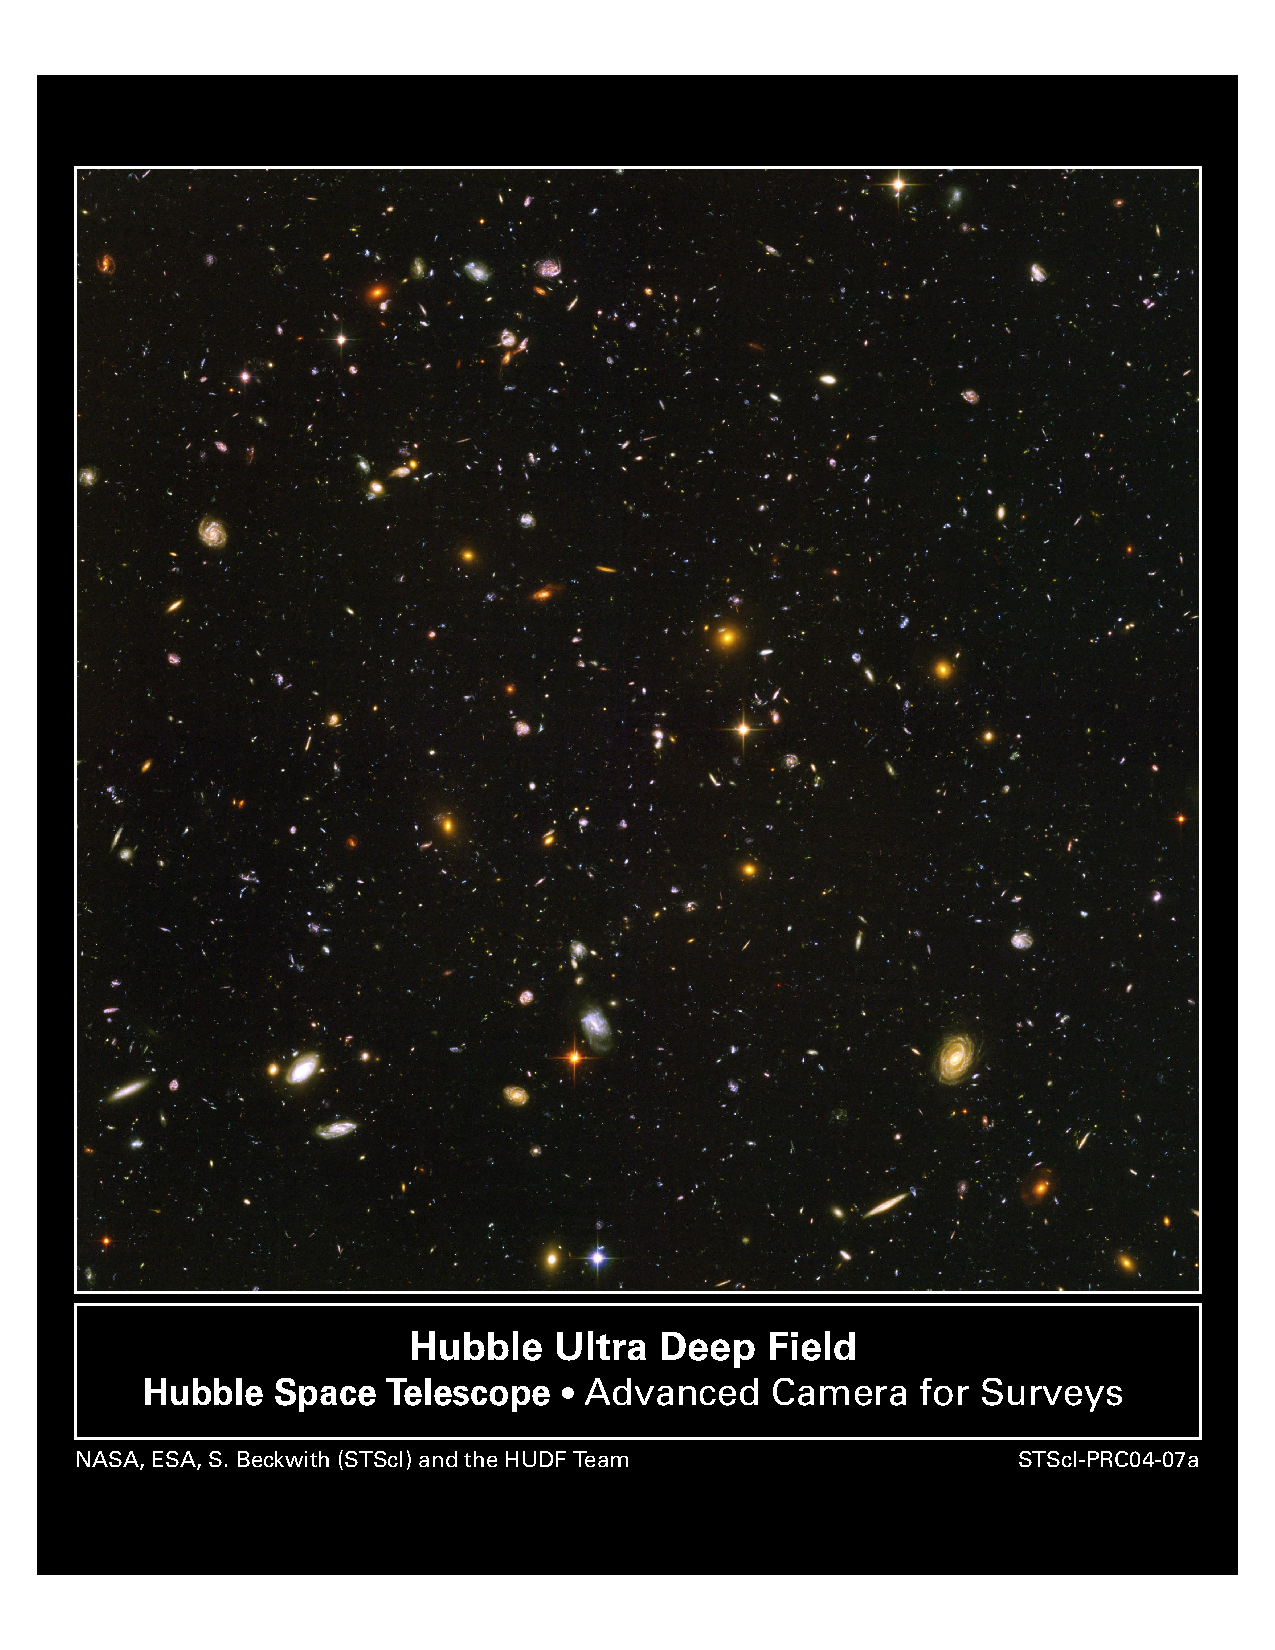
\includegraphics[scale=0.45,trim={40 400 40 80},clip]{../beamer/hs-2004-07-a-pdf}
\caption{Hubble Ultra Deep Field \cite{HUDF}}
\label{fig:hs-2004-07-a-pdf}
\end{figure}

\IEEEPARstart{D}{ie} Unterscheidung ob ein Objekt ein Stern, eine Galaxie oder etwas Unbekanntes ist, lässt sich
mittels Data Mining Techniken Automatisieren. In dem Paper \cite{o2009star} von Peter J. O’Keefe und weiteren
wird dieser Vorgehen beschrieben. Jedem sichtbarem Objekt werden 9 Attribute zugeordnet, die aus den 
$i$-Band Versionen der Aufnahmen extrahiert werden. Die Attribute bestehen aus der Leuchtkraft und 8 weiteren Lichteigenschaften
und werden zu einer Zahl, genannt \emph{stellary}, zwischen 0 und 1 ausgewertet. Das Intervall $0.0$--$0.1$ repräsentiert eine Galaxie, $0.9$--$1.0$ einen 
Stern und sonst ist das Objekt unbekannt aber könnte trotzdem ein Stern oder Galaxie sein. In Tabelle \ref{Erkennungswahrscheinlichkeiten} sind die Erkennungswahrscheinlichkeiten einiger 
Data Mining Algorithmen für die Klassifizierung von stellaren Objekten aufgelistet.

\begin{table}[!h]
\centering
\label{Erkennungswahrscheinlichkeiten}
\caption{Erkennung \cite{o2009star}}
\begin{tabular}{l|l}
Name & Erkennung\\ \hline
Random Forest & $82,89\%$ \\
Decision Tree & $80,68\%$ \\
Artificial Neural Network & $75.82\%$ \\
Support Vector Machines & $37,82\%$
\end{tabular}
\end{table}

\IEEEPARstart{D}{as} Paper \cite{wu2008top} von Xindong Wu und weiteren mit dem Titel \emph{Top 10 Algorithms in Data Mining} wurde 
im Dezember 2006 für die \emph{IEEE International Conference on Data Mining} erstellt, behandelt die zum damaligen 
Zeitpunkt wichtigsten Algorithmen fürs Data Mining und dient als Quelle für das gesamte Paper. Die Auswahl der einzelnen Algorithmen erfolge, indem jeder 
Preisträger eines \emph{ACM KDD Innovation Awards} oder eines \emph{IEEE ICDM Research Contributions Awards} jeweils 
10 Algorithmen nominierte. Aus diesen Nominierten wurden nur die zur Abstimmung zugelassen, die mindestens 50 
Referenzierungen in \emph{Google Scholar} erreichen. Eine vollständige Liste der Kandidaten ist unter \url{http://www.cs.uvm.edu/~icdm/algorithms/CandidateList.shtml}
zu finden. In der Tabelle \ref{top10} werden die 10 besten Algorithmen genannt.

\begin{table}
\centering
\caption{Top 10 Algorithmen \cite{wu2008top}}
\begin{tabular}{r|l|l}
Platz & Name & Art\\ \hline
1.& C4.5 & Classification\\
2.& k-means & Clustering\\
3.& Suport Vector Machines & Classification\\
4.& Apriori & Association\\
5.& EM Algorithm & Classification\\
6.& PageRank & Link Mining\\
7.& AdaBoost & Classification\\
8.& k-nearest neighbor & Classification\\
9.& Naive Bayes & Classification\\
10.& CART & Classification
\end{tabular}
\label{top10}
\end{table}

\section{Data Mining}

\IEEEPARstart{D}{er} Begriff Data Mining wird im Deutschen für den gesamten Prozess des \emph{Knowledge Discovery in Databases} (KDD) 
verwendet. Dies ist jedoch falsch, da Data Mining nur einen Teil des KDD einnimmt. Dies ist in Abbildung \ref{kdd} zu sehen. 
Für KDD werden zuerst die Daten homogenisiert und dann mittels eines Data Mining Algorithmus verarbeitet, sodass \enquote{Wissen} 
entsteht. 

 \begin{figure}[!t]
  \centering
  \hspace{-4em}\includegraphics[page=5,scale=0.6,trim={51 500 65 86},clip]{../beamer/dm_fayyad.pdf}
  \caption{KDD nach Fayyad \cite{fayyad1996data}}
  \label{kdd}
  \end{figure}
\IEEEPARstart{D}{ata Mining} wird in der Forschung, Vermarktung, Medizin, (Wetter-) Vorhersagen,
Betrugsaufklärung usw. eingesetzt. Die Idee von KKD ist \emph{Wissen} durch \emph{Daten} und wird nach Fayyad \cite{fayyad1996data} wie folgt definiert: \begin{quote}
Knowledge Discovery in Databases describes the non-trivial process of identifying valid, novel, potentially useful, and ultimately understandable
Articles patterns in data.
\end{quote} 
 
 \subsection{Clustering-Algorithmen}
 \IEEEPARstart{D}{ie} Kategorie der Clustering-Algorithmen beschreibt Algorithmen, 
 die Daten unbekannten Klassen, den so genannten \emph{Clustern} (Abschnitt \ref{cluster}), zu ordnen. Damit ist die Grundidee 
 das Finden eines Algorithmus, der Objekte gruppiert. Diese Gruppierung wird mit Hilfe
 einer \emph{Distanzfunktion} (Abschnitt \ref{distanzfunktion}) erreicht, die die Ähnlichkeit zwischen Objekten numerisch ermittelt.
 Alle Clustering-Algorithmen arbeiten mit Heuristiken, da das Clustering NP-Vollständig ist.

\subsubsection{Cluster} \label{cluster}

\IEEEPARstart{D}{ie} Gestalt und Form der Cluster ist in den einzelnen Algorithmen sehr 
unterschiedlich. So gibt es Algorithmen bei denen die Cluster hierarchisch verschachtelt
sind, das so genannte Flache- oder Hierarchische-Clustering. Es existiert ebenfalls das Hard- 
und Soft-Clustering, bei denen Objekte zu einem oder mehreren von einander unabhängigen Clustern 
zu geordnet sind. Bei allen Algorithmen ist die Anzahl der Cluster begrenzt durch direkte Festlegung 
der Anzahl oder durch eine Angegebene ausreichende Qualität der einzelnen Cluster. Die Cluster-Qualität
ist ebenfalls nie genau definiert, jedoch kann man diese recht ungenau beschreiben durch, Anzahl der 
einzelnen Objekte die einem Cluster angehören, Größe des maximalen Unähnlichkeit eines Objektes zu seinem Cluster oder
das vermeiden von \emph{Lücken} im Cluster. In Abbildung \ref{p4 k-means} sind beispielhaft zwei Cluster (rot / blau) 
und die Clusterzentren (schwarz) des k-means Algorithmus (Abschnitt \ref{k-means}) gezeigt. Vergleiche das Buch \cite{ester2000knowledge} 
und die Vorlesung \cite{dwh}.



\subsubsection{Distanzfunktion} \label{distanzfunktion}
\IEEEPARstart{D}{ie} Distanzfunktion bestimmt den Abstandsvektor zwischen zwei Objekten. Statt einer Distanzfunktion
wird manchmal auch eine Ähnlichkeits- bzw. Simulierungsfunktion benutzt, jedoch sind in diesem
Fall die Werte invertiert zu betrachten. Der Gebrauch von Distanzfunktionen hat sich jedoch durch
gesetzt, da alle Rechnungen nummerisch stabiler sind, weil bei der Bedingung \ref{dist2} mit $\vec{0}$ 
statt $\vec{\infty}$ gerechnet wird. Jedes Objekt $o_i = (a_1, \ldots, a_n)$ besteht aus $n$ Attributen, jedes 
Attribut ist ein Nummerisches oder Kategorisches- oder anders artiges-Attribut und besitzt für sich selbst 
spezielle Distanzfunktionen. Die Bedingungen \ref{bed1} -- \ref{bed3} müssen für jede 
Distanzfunktion gelten. Wenn die Bedingung \ref{bed4} gilt, handelt es sich um eine Metrik.
\begin{align}
\dist(o_1, o_2) &= d \in R^{n\geq 0} \label{bed1}\\
\dist(o_1, o_2) &= 0 \Leftrightarrow o_1 = o_2 \label{bed2}\\
\dist(o_1, o_2) &= \dist(o_2, o_1) \mbox{ (Symmetrie)} \label{bed3}\\
\dist(o_1, o_3) &\leq \dist(o_1, o_2) + \dist(o_2, o_3) \label{bed4}
\end{align} 

\IEEEPARstart{F}{ür} Nummerische-Attribute existieren die beispielhaften Distanzfunktionen (\ref{dist1} -- \ref{dist4}) und für 
Kategorische-Attribute existiert die Summe der Unterschiede (\ref{dist5}). 
Allerdings existieren nicht nur Kategorische- und Nummerische-Attribute sondern ebenfalls 
Textuelle-Attribute usw. die dazu gehörigen Distanzfunktionen erfüllen genauso mindestens die
Bedingungen \ref{bed1} -- \ref{bed3}.
{
\setlength{\jot}{0pt}
\begin{align}
\intertext{Euklidische-Distanz:} 
\dist(x,y) &= \sqrt{(x_1 - y_1)^2 + \ldots + (x_n - y_n)^2}\label{dist1}\\
\intertext{Manhattan-Distanz:}
\dist(x,y) &= |x_1 - y_1| + \ldots + |x_n - y_n|\label{dist2}\\
\intertext{Maximum-Metrik:} 
\dist(x,y) &= \max\big(|x_1 - y_1| + \ldots + |x_n - y_n|\big)\label{dist3}\\
\intertext{Alg. $L_p$-Metrik:}
\dist(x,y) &= \sqrt[p]{\sum\limits_{i=1}^{d}{(x_i-y_i)^p}}\label{dist4}\\
\intertext{Summe der Unterschiede:} 
 \dist(x,y) &= \sum\limits_{i=1}^{a}\delta(x_i, y_i)\label{dist5}\\
 \delta(x_i, y_i) &= \begin{cases}
 0 \mbox{ wenn } (x_i = y_i)\\
 1 \mbox{ wenn } (x_i \neq y_i)
 \end{cases} 
 \end{align} 
 }
\subsubsection{k-means} \label{k-means}
\IEEEPARstart{D}{er} k-means, oder auch Lloyd's Algorithmus genannt, gehört zu den Clustering-Algorithmen und basiert auf 
einem harten flachen Clustering. Die Objekte $o_i$ werden als ein Vektor aus dem 
Vektorraum $R^n$ interpretiert. Ein Cluster $A = \{o_1, \ldots o_i\}$ ist eine Menge
von Objekten $o_i$ und dessen Zentrum ist wie folgt definiert: 
$\mu(A) = \frac{l}{m}\sum\limits_{i=l}^{m}o_i$. Ein Cluster besitzt eine hohe Güte, 
wenn $\RSS\,(A) = \sum\limits_{i=l}^{m}\big\|d_i - \mu(A)\big\|^2$ minimal ist. 
Das gesamte Clustering ist optimal, wenn $\RSS\,(A_l, \ldots, A_k) = \sum\limits_{j=l}^{k}\,\RSS\,(A_j)$ minimal ist. 

\begin{figure}[!t]
\centering
\subfigure[Phase 1 -- 3]{\scalebox{0.5}{\tikzstyle{none}=[inner sep=0pt]
\definecolor{hexcolor0x0074ff}{rgb}{0.000,0.455,1.000}
\definecolor{hexcolor0xff2615}{rgb}{1.000,0.149,0.082}

\definecolor{myblack}{rgb}{0.000,0.000,0.000}
\definecolor{mywhite}{rgb}{1.000,1.000,1.000}

\tikzstyle{sp}=[circle,fill=myblack,draw=myblack, scale=1]
\tikzstyle{setA}=[circle,fill=hexcolor0x0074ff,draw=myblack]
\tikzstyle{setB}=[circle,fill=hexcolor0xff2615,draw=myblack]
\tikzstyle{setC}=[circle,fill=mywhite,draw=myblack]
\tikzstyle{node}=[circle,fill=mywhite,draw=myblack,scale=.1]


\begin{tikzpicture}
	%\begin{pgfonlayer}{nodelayer}
		\node [style=setC] (0) at (-1.75, 1.75) {};
		\node [style=setC] (1) at (-3, 0.5) {};
		\node [style=setC] (2) at (0,2) {};
		\node [style=setC] (3) at (-1.25, 0.75) {};
		\node [style=setC] (4) at (-2.25, 1) {};
		\node [style=setC] (5) at (-3.25, 1.75) {};
		\node [style=setC] (6) at (-1.75, 2.75) {};
		\node [style=setC] (7) at (-1, 1.5) {};
		\node [style=setC] (8) at (2.25, 1.5) {};
		\node [style=setC] (9) at (1.25, 0.75) {};
		\node [style=setC] (10) at (2.75, -0.25) {};
		\node [style=setC] (11) at (0,-0.5) {};
		\node [style=setC] (12) at (3.25, 1) {};
		\node [style=setC] (13) at (2, 0.5) {};
		\node [style=setC] (14) at (2.5, -1.5) {};
		\node [style=setC] (15) at (-1,-1.5) {};
		\node [style=setC] (16) at (1.25, -1.75) {};
		\node [style=setC] (17) at (1.75, -0.25) {};
		\node [style=setC] (18) at (-2.25, -0.25) {};
		\node [style=setC] (19) at (1.75, 1) {};

\node [sp] at (-1,-0.5) {};
\node [sp] at (1,1.5) {};
\end{tikzpicture}}\label{p1-3 k-means}}
\subfigure[Phase 4]{\scalebox{0.5}{\tikzstyle{none}=[inner sep=0pt]
\definecolor{hexcolor0x0074ff}{rgb}{0.000,0.455,1.000}
\definecolor{hexcolor0xff2615}{rgb}{1.000,0.149,0.082}

\definecolor{myblack}{rgb}{0.000,0.000,0.000}
\definecolor{mywhite}{rgb}{1.000,1.000,1.000}

\tikzstyle{sp}=[circle,fill=myblack,draw=myblack, scale=1]
\tikzstyle{setA}=[circle,fill=hexcolor0x0074ff,draw=myblack]
\tikzstyle{setB}=[circle,fill=hexcolor0xff2615,draw=myblack]
\tikzstyle{setC}=[circle,fill=mywhite,draw=myblack]
\tikzstyle{node}=[circle,fill=mywhite,draw=myblack,scale=.1]


\begin{tikzpicture}
		\node [style=setA] (0) at (-1.75, 1.75) {};
		\node [style=setB] (1) at (-3, 0.5) {};
		\node [style=setA] (2) at (0,2) {};
		\node [style=setB] (3) at (-1.25, 0.75) {};
		\node [style=setB] (4) at (-2.25, 1) {};
		\node [style=setB] (5) at (-3.25, 1.75) {};
		\node [style=setA] (6) at (-1.75, 2.75) {};
		\node [style=setA] (7) at (-1, 1.5) {};
		\node [style=setA] (8) at (2.25, 1.5) {};
		\node [style=setA] (9) at (1.25, 0.75) {};
		\node [style=setA] (10) at (2.75, -0.25) {};
		\node [style=setB] (11) at (0,-0.5) {};
		\node [style=setA] (12) at (3.25, 1) {};
		\node [style=setA] (13) at (2, 0.5) {};
		\node [style=setB] (14) at (2.5, -1.5) {};
		\node [style=setB] (15) at (-1,-1.5) {};
		\node [style=setB] (16) at (1.25, -1.75) {};
		\node [style=setA] (17) at (1.75, -0.25) {};
		\node [style=setB] (18) at (-2.25, -0.25) {};
		\node [style=setA] (19) at (1.75, 1) {};

\node [sp] (v1) at (-1,-0.5) {};
\node [sp] (v2) at (1,1.5) {};
\draw  (3) edge (v1);
\draw  (11) edge (v1);
\draw  (15) edge (v1);
\draw  (18) edge (v1);
\draw  (4) edge (v1);
\draw  (1) edge (v1);
\draw  (5) edge (v1);
\draw  (16) edge (v1);
\draw  (14) edge (v1);
\draw  (6) edge (v2);
\draw  (0) edge (v2);
\draw  (7) edge (v2);
\draw  (2) edge (v2);
\draw  (9) edge (v2);
\draw  (19) edge (v2);
\draw  (8) edge (v2);
\draw  (12) edge (v2);
\draw  (13) edge (v2);
\draw  (17) edge (v2);
\draw  (10) edge (v2);
\end{tikzpicture}}\label{p4 k-means}}
\subfigure[Phase 5]{\scalebox{0.5}{\tikzstyle{none}=[inner sep=0pt]
\definecolor{hexcolor0x0074ff}{rgb}{0.000,0.455,1.000}
\definecolor{hexcolor0xff2615}{rgb}{1.000,0.149,0.082}

\definecolor{myblack}{rgb}{0.000,0.000,0.000}
\definecolor{mywhite}{rgb}{1.000,1.000,1.000}

\tikzstyle{sp}=[circle,fill=myblack,draw=myblack, scale=1]
\tikzstyle{setA}=[circle,fill=hexcolor0x0074ff,draw=myblack]
\tikzstyle{setB}=[circle,fill=hexcolor0xff2615,draw=myblack]
\tikzstyle{setC}=[circle,fill=mywhite,draw=myblack]
\tikzstyle{node}=[circle,fill=mywhite,draw=myblack,scale=.1]


\begin{tikzpicture}
		\node [style=setA] (0) at (-1.75, 1.75) {};
		\node [style=setB] (1) at (-3, 0.5) {};
		\node [style=setA] (2) at (0,2) {};
		\node [style=setB] (3) at (-1.25, 0.75) {};
		\node [style=setB] (4) at (-2.25, 1) {};
		\node [style=setB] (5) at (-3.25, 1.75) {};
		\node [style=setA] (6) at (-1.75, 2.75) {};
		\node [style=setA] (7) at (-1, 1.5) {};
		\node [style=setA] (8) at (2.25, 1.5) {};
		\node [style=setA] (9) at (1.25, 0.75) {};
		\node [style=setA] (10) at (2.75, -0.25) {};
		\node [style=setB] (11) at (0,-0.5) {};
		\node [style=setA] (12) at (3.25, 1) {};
		\node [style=setA] (13) at (2, 0.5) {};
		\node [style=setB] (14) at (2.5, -1.5) {};
		\node [style=setB] (15) at (-1,-1.5) {};
		\node [style=setB] (16) at (1.25, -1.75) {};
		\node [style=setA] (17) at (1.75, -0.25) {};
		\node [style=setB] (18) at (-2.25, -0.25) {};
		\node [style=setA] (19) at (1.75, 1) {};

\node [none] (v2) at (-1,-0.5) {};
\node [none] (v3) at (1,1.5) {};

\node [sp] (v1) at (-1.5,0) {};
\node [sp] (v4) at (1.5,1) {};
\draw  (v2) edge (v1);
\draw  (v3) edge (v4);
\end{tikzpicture}}\label{p5 k-means}}
\subfigure[Phase 6]{\scalebox{0.5}{\tikzstyle{none}=[inner sep=0pt]
\definecolor{hexcolor0x0074ff}{rgb}{0.000,0.455,1.000}
\definecolor{hexcolor0xff2615}{rgb}{1.000,0.149,0.082}

\definecolor{myblack}{rgb}{0.000,0.000,0.000}
\definecolor{mywhite}{rgb}{1.000,1.000,1.000}

\tikzstyle{sp}=[circle,fill=myblack,draw=myblack, scale=1]
\tikzstyle{setA}=[circle,fill=hexcolor0x0074ff,draw=myblack]
\tikzstyle{setB}=[circle,fill=hexcolor0xff2615,draw=myblack]
\tikzstyle{setC}=[circle,fill=mywhite,draw=myblack]
\tikzstyle{node}=[circle,fill=mywhite,draw=myblack,scale=.1]

\begin{tikzpicture}
		\node [style=setB] (0) at (-1.75, 1.75) {};
		\node [style=setB] (1) at (-3, 0.5) {};
		\node [style=setA] (2) at (0,2) {};
		\node [style=setB] (3) at (-1.25, 0.75) {};
		\node [style=setB] (4) at (-2.25, 1) {};
		\node [style=setB] (5) at (-3.25, 1.75) {};
		\node [style=setB] (6) at (-1.75, 2.75) {};
		\node [style=setB] (7) at (-1, 1.5) {};
		\node [style=setA] (8) at (2.25, 1.5) {};
		\node [style=setA] (9) at (1.25, 0.75) {};
		\node [style=setA] (10) at (2.75, -0.25) {};
		\node [style=setB] (11) at (0,-0.5) {};
		\node [style=setA] (12) at (3.25, 1) {};
		\node [style=setA] (13) at (2, 0.5) {};
		\node [style=setA] (14) at (2.5, -1.5) {};
		\node [style=setB] (15) at (-1,-1.5) {};
		\node [style=setA] (16) at (1.25, -1.75) {};
		\node [style=setA] (17) at (1.75, -0.25) {};
		\node [style=setB] (18) at (-2.25, -0.25) {};
		\node [style=setA] (19) at (1.75, 1) {};
		
\node [sp] (v1) at (-1.5,0) {};
\node [sp] (v4) at (1.5,1) {};

\draw  (v1) edge (3);
\draw  (7) edge (v1);
\draw  (0) edge (v1);
\draw  (4) edge (v1);
\draw  (1) edge (v1);
\draw  (5) edge (v1);
\draw  (6) edge (v1);
\draw  (18) edge (v1);
\draw  (15) edge (v1);
\draw  (11) edge (v1);
\draw  (2) edge (v4);
\draw  (9) edge (v4);
\draw  (19) edge (v4);
\draw  (8) edge (v4);
\draw  (12) edge (v4);
\draw  (13) edge (v4);
\draw  (10) edge (v4);
\draw  (17) edge (v4);
\draw  (16) edge (v4);
\draw  (14) edge (v4);
\end{tikzpicture}}\label{p6 k-means}}
\caption{k-means}
\label{k-means 1-6}
\end{figure}

Der Algorithmus ist wie folgt:
\begin{enumerate}
\item Selektiere zufällig $k$ Zentren als Startwert
\item Erstelle $k$ leere Cluster
\item Weise jedem Cluster einen Zentren zu (siehe Abbildung \ref{p1-3 k-means})
\item Weise jedem Datenvektor den Cluster mit dem nächstem Zentrum zu (siehe Abbildung \ref{p4 k-means})
\item Berechne den Zentrum jedes Clusters neu (siehe Abbildung \ref{p5 k-means})
\item Teste, ob die Qualität des Clusterings ausreicht, sonst gehe zu 2. (siehe Abbildung \ref{p6 k-means})
\end{enumerate}


 \subsection{Classification-Algorithmen}
 \IEEEPARstart{B}{ei} der Kategorie der Classification-Algorithmen sind anders 
 als bei den Clustering-Algorithmen die genauen Klassen in die 
 eingruppiert wird bereits bekannt. Der einzige weitere große 
 Unterschied zwischen beiden Kategorien ist, das bei den 
 Classification-Algorithmen Trainingsdaten (siehe Abschnitt \ref{training}) verwendet werden. 
 Die verwendeten Distanzfunktionen sind mit denen fürs Clustering (Abschnitt \ref{distanzfunktion}) vergleichbar.
 
 \subsubsection{Training}\label{training}
 \IEEEPARstart{T}{rainingsdaten} sind eine Menge von Objekten $O = \{o_1, \ldots, o_n\}$
 bei denen die Klassen $C = \{c_1, \ldots, c_m\}$ bereits bekannt sind oder manuell 
 ermittelt wurden. Für die Objekte gelten die gleichen Eigenschaften wie beim Clustering 
 (siehe Abschnitt \ref{distanzfunktion}). Um das Training zu verdeutlichen wird ein Beispiel 
 aus dem Buch \cite{ester2000knowledge} verwendet. Dabei sind in Tabelle 
 \ref{trainingdata} Objekte mit ihren Attributen und der jeweils zugeordneten Klasse gezeigt. 
 Aus diesen Trainingsdaten wird der, in Listing \ref{dt} als Bedingung formulierte, Entscheidungsbaum
 erzeugt. Mit Hilfe dieses Entscheidungsbaums können unklassifizierte Objekte klassifiziert werden. 

\begin{table}[!h]
\caption{Beispiel Daten}
\centering
\begin{tabular}{l|l|l}\hline
Alter	& Autotyp	& Risikoklasse \\\hline
23	& Familie	& Hoch\\
17	& Sport		& Hoch\\
43	& Sport		& Hoch\\
68	& Familie	& Niedrig\\
32	& LKW		& Niedrig
\end{tabular}
\label{trainingdata}
\end{table}
\begin{lstlisting}[caption={Entscheidungsbaum},label=dt,frame=single]
if Alter > 50 then Risikoklasse = Niedrig
if Alter <= 50 and Autotyp = LKW 
  then Risikoklasse = Niedrig
  else Risikoklasse = Hoch
\end{lstlisting}

\subsubsection{Support Vector Machines}
\IEEEPARstart{B}{ei} den Support Vector Machines (SVM) handelt es sich eigentlich 
um einen Algorithmus des \emph{Statistical Learning} aber diese Algorithmen sind eine
Unterkategorie der Classification. Der SVM kann eine Menge von Objekten nur in zwei 
disjunkte Teilmengen spalten. Zwischen den beiden Teilmengen der Trainingsdaten wird 
eine Hyperplane im $n$-dimensionalen Vektorraum erstellt. Der Abstand zwischen der
Hyperebene und den Begrenzungsobjekten der Teilmengen, die so genannten Supportvektoren, 
ist maximal. Dieser Abstand wird mittels Differenzfunktionen wie beim Clustering 
(siehe Abschnitt \ref{distanzfunktion}) ermittelt.

\begin{figure}[!t]
\centering
\subfigure[Gesucht]{\scalebox{0.42}{\tikzstyle{none}=[inner sep=0pt]
\definecolor{hexcolor0x0074ff}{rgb}{0.000,0.455,1.000}
\definecolor{hexcolor0xff2615}{rgb}{1.000,0.149,0.082}

\definecolor{myblack}{rgb}{0.000,0.000,0.000}
\definecolor{mywhite}{rgb}{1.000,1.000,1.000}

\tikzstyle{setA}=[circle,fill=hexcolor0x0074ff,draw=myblack]
\tikzstyle{setB}=[circle,fill=hexcolor0xff2615,draw=myblack]
\tikzstyle{node}=[circle,fill=mywhite,draw=myblack,scale=.1]


\begin{tikzpicture}
	%\begin{pgfonlayer}{nodelayer}
		\node [style=setA] (0) at (-1.75, 1.75) {};
		\node [style=setA] (1) at (-3, 0.5) {};
		\node [style=setA] (2) at (0,2) {};
		\node [style=setA] (3) at (-1.25, 0.75) {};
		\node [style=setA] (4) at (-2.25, 1) {};
		\node [style=setA] (5) at (-3.25, 1.75) {};
		\node [style=setA] (6) at (-1.75, 2.75) {};
		\node [style=setA] (7) at (-1, 1.5) {};
		\node [style=setB] (8) at (2.25, 1.5) {};
		\node [style=setB] (9) at (1.25, 0.75) {};
		\node [style=setB] (10) at (2.75, -0.25) {};
		\node [style=setB] (11) at (0,-0.5) {};
		\node [style=setB] (12) at (3.25, 1) {};
		\node [style=setB] (13) at (2, 0.5) {};
		\node [style=setB] (14) at (2.5, -1.5) {};
		\node [style=setB] (15) at (-1,-1.5) {};
		\node [style=setB] (16) at (1.25, -1.75) {};
		\node [style=setB] (17) at (1.75, -0.25) {};
		\node [style=setA] (18) at (-2.25, -0.25) {};
		\node [style=setB] (19) at (1.75, 1) {};
		\node [style=node] (20) at (1,3.5) {};
		\node [style=node] (21) at (-2,-3.5) {};
		\node [style=node] (22) at (-4.25, -1.5) {};
		\node [style=node] (23) at (4.25, 2.75) {};
		\node [style=node] (24) at (2.5, 3.5) {};
		\node [style=node] (25) at (-4.25, -3.5) {};
	%\end{pgfonlayer}
	%\begin{pgfonlayer}{edgelayer}
		\draw [ultra thick] (22) to (23);
		\draw [ultra thick] (20) to (21);
		\draw [ultra thick] (25) to (24);
	%\end{pgfonlayer}
\node [none] (v1) at (-3.5,3) {};
\node [none] (v2) at (-5,-3.5) {};
\node [none] (v3) at (5,4) {};
\node [none] (v4) at (2,-3.5) {};
\draw [ultra thick] (v1) edge (v2);
\draw [ultra thick] (v3) edge (v4);
\end{tikzpicture}}\label{hyperplane gesucht}}
\subfigure[Gefunden]{\scalebox{0.42}{\tikzstyle{none}=[inner sep=0pt]
\definecolor{hexcolor0x0074ff}{rgb}{0.000,0.455,1.000}
\definecolor{hexcolor0xff2615}{rgb}{1.000,0.149,0.082}

\definecolor{myblack}{rgb}{0.000,0.000,0.000}
\definecolor{mywhite}{rgb}{1.000,1.000,1.000}

\tikzstyle{setA}=[circle,fill=hexcolor0x0074ff,draw=myblack]
\tikzstyle{setB}=[circle,fill=hexcolor0xff2615,draw=myblack]
\tikzstyle{node}=[circle,fill=mywhite,draw=myblack,scale=.1]


\begin{tikzpicture}
	%\begin{pgfonlayer}{nodelayer}
		\node [style=setA] (0) at (-1.75, 1.75) {};
		\node [style=setA] (1) at (-3, 0.5) {};
		\node [style=setA] (2) at (0,2) {};
		\node [style=setA] (3) at (-1.25, 0.75) {};
		\node [style=setA] (4) at (-2.25, 1) {};
		\node [style=setA] (5) at (-3.25, 1.75) {};
		\node [style=setA] (6) at (-1.75, 2.75) {};
		\node [style=setA] (7) at (-1, 1.5) {};
		\node [style=setB] (8) at (2.25, 1.5) {};
		\node [style=setB] (9) at (1.25, 0.75) {};
		\node [style=setB] (10) at (2.75, -0.25) {};
		\node [style=setB] (11) at (0,-0.5) {};
		\node [style=setB] (12) at (3.25, 1) {};
		\node [style=setB] (13) at (2, 0.5) {};
		\node [style=setB] (14) at (2.5, -1.5) {};
		\node [style=setB] (15) at (-1,-1.5) {};
		\node [style=setB] (16) at (1.25, -1.75) {};
		\node [style=setB] (17) at (1.75, -0.25) {};
		\node [style=setA] (18) at (-2.25, -0.25) {};
		\node [style=setB] (19) at (1.75, 1) {};
		\node [style=node] (20) at (1.5, 3.5) {};
		\node [style=node] (21) at (-4.5,-3) {};
		\node [style=node] (22) at (3.5, 3.5) {};
		\node [style=node] (23) at (-2.5,-3) {};
		\node [style=node] (24) at (-3.5, -3) {};
		\node [style=node] (25) at (2.5, 3.5) {};
	%\end{pgfonlayer}
	%\begin{pgfonlayer}{edgelayer}
	\filldraw[thick,fill=green,fill opacity=0.4] (20.center) -- (21.center) -- (23.center) -- (22.center) -- cycle;

		%\draw (21) to (20);
		%\draw (23) to (22);
		\draw [ultra thick] (24) to (25);
	%\end{pgfonlayer}
\end{tikzpicture}}\label{hyperplane gefunden}}
\subfigure[Einordnung]{\scalebox{0.49}{\tikzstyle{none}=[inner sep=0pt]
\definecolor{hexcolor0x0074ff}{rgb}{0.000,0.455,1.000}
\definecolor{hexcolor0xff2615}{rgb}{1.000,0.149,0.082}

\definecolor{myblack}{rgb}{0.000,0.000,0.000}
\definecolor{mywhite}{rgb}{1.000,1.000,1.000}

\tikzstyle{setA}=[circle,fill=hexcolor0x0074ff,draw=myblack]
\tikzstyle{setB}=[circle,fill=hexcolor0xff2615,draw=myblack]
\tikzstyle{setc}=[circle,fill=mywhite,draw=myblack]
\tikzstyle{node}=[circle,fill=mywhite,draw=myblack,scale=.1]


\begin{tikzpicture}
	%\begin{pgfonlayer}{nodelayer}
		\node [style=setA] (0) at (-1.75, 1.75) {};
		\node [style=setA] (1) at (-3, 0.5) {};
		\node [style=setA] (2) at (0,2) {};
		\node [style=setA] (3) at (-1.25, 0.75) {};
		\node [style=setA] (4) at (-2.25, 1) {};
		\node [style=setA] (5) at (-3.25, 1.75) {};
		\node [style=setA] (6) at (-1.75, 2.75) {};
		\node [style=setA] (7) at (-1, 1.5) {};
		\node [style=setB] (8) at (2.25, 1.5) {};
		\node [style=setB] (9) at (1.25, 0.75) {};
		\node [style=setB] (10) at (2.75, -0.25) {};
		\node [style=setB] (11) at (0,-0.5) {};
		\node [style=setB] (12) at (3.25, 1) {};
		\node [style=setB] (13) at (2, 0.5) {};
		\node [style=setB] (14) at (2.5, -1.5) {};
		\node [style=setB] (15) at (-1,-1.5) {};
		\node [style=setB] (16) at (1.25, -1.75) {};
		\node [style=setB] (17) at (1.75, -0.25) {};
		\node [style=setA] (18) at (-2.25, -0.25) {};
		\node [style=setB] (19) at (1.75, 1) {};
		\node [style=node] (20) at (1.5, 3.5) {};
		\node [style=node] (21) at (-4.5,-3) {};
		\node [style=node] (22) at (3.5, 3.5) {};
		\node [style=node] (23) at (-2.5,-3) {};
		\node [style=node] (24) at (-3.5, -3) {};
		\node [style=node] (25) at (2.5, 3.5) {};
	%\end{pgfonlayer}
	%\begin{pgfonlayer}{edgelayer}
	
	%\end{pgfonlayer}
\node [setc] at (0,0.5) {};
\node [setc] at (1,1.5) {};
\node [setc] at (2,2.5) {};
\node [setc] at (2.5,2) {};
\node [setc] at (2.5,1) {};
\node [setc] at (0.5,-0.5) {};
\node [setc] at (1.5,-1.5) {};
\node [setc] at (2.5,-1) {};
\node [setc] at (3,0.5) {};
\node [setc] at (1,-0.5) {};
\node [setc] at (1,0.5) {};
\node [setc] at (-1,-0.5) {};
\node [setc] at (0,-1) {};
\node [setc] at (-2,-2) {};
\node [setc] at (-1.5,-2) {};
\node [setc] at (0,-1.5) {};
\node [setc] at (1,-1) {};
\node [setc] at (0,1.5) {};
\node [setc] at (1,2.5) {};
\node [setc] at (0.5,3.5) {};
\node [setc] at (-1.5,0) {};
\node [setc] at (-0.5,0.5) {};
\node [setc] at (-2.5,-1) {};
\node [setc] at (-4,-0.5) {};
\node [setc] at (-4,-2) {};
\node [setc] at (-3,-1.5) {};
\node [setc] at (-3,-0.5) {};
\node [setc] at (-4,1) {};
\node [setc] at (-1,2.5) {};
\node [setc] at (0,2.5) {};
\node [setc] at (-0.5,3) {};
\node [setc] at (1.5,3) {};
\node [setc] at (2.5,3) {};
\node [setc] at (-0.5,1) {};
\node [setc] at (0.5,1) {};
\node [setc] at (-2,-1) {};
\node [setc] at (-1.5,-1) {};
\node [setc] at (-3.5,-2) {};
\node [setc] at (-2.5,-2.5) {};

\filldraw[thick,fill=green,fill opacity=0.4] (20.center) -- (21.center) -- (23.center) -- (22.center) -- cycle;

		%\draw (21) to (20);
		%\draw (23) to (22);
		\draw [ultra thick] (24) to (25);
\end{tikzpicture}}\label{einordnung}}
\subfigure[Ungültige Daten]{\scalebox{0.49}{\tikzstyle{none}=[inner sep=0pt]
\definecolor{hexcolor0x0074ff}{rgb}{0.000,0.455,1.000}
\definecolor{hexcolor0xff2615}{rgb}{1.000,0.149,0.082}

\definecolor{myblack}{rgb}{0.000,0.000,0.000}
\definecolor{mywhite}{rgb}{1.000,1.000,1.000}

\tikzstyle{setA}=[circle,fill=hexcolor0x0074ff,draw=myblack]
\tikzstyle{setB}=[circle,fill=hexcolor0xff2615,draw=myblack]
\tikzstyle{node}=[circle,fill=mywhite,draw=myblack,scale=.1]


\begin{tikzpicture}
	%\begin{pgfonlayer}{nodelayer}
		\node [style=setA] (0) at (-1.75, 1.75) {};
		\node [style=setA] (1) at (-3, 0.5) {};
		\node [style=setA] (2) at (0,2) {};
		\node [style=setA] (3) at (1,0) {};
		\node [style=setA] (4) at (-2.25, 1) {};
		\node [style=setA] (5) at (-3.25, 1.75) {};
		\node [style=setA] (6) at (-1.75, 2.75) {};
		\node [style=setA] (7) at (-1, 1.5) {};
		\node [style=setB] (8) at (2.25, 1.5) {};
		\node [style=setB] (9) at (1.25, 0.75) {};
		\node [style=setB] (10) at (2.75, -0.25) {};
		\node [style=setB] (11) at (-1,0.5) {};
		\node [style=setB] (12) at (3.25, 1) {};
		\node [style=setB] (13) at (2, 0.5) {};
		\node [style=setB] (14) at (2.5, -1.5) {};
		\node [style=setB] (15) at (-1,-1.5) {};
		\node [style=setB] (16) at (1.25, -1.75) {};
		\node [style=setB] (17) at (1.75, -0.25) {};
		\node [style=setA] (18) at (-2.25, -0.25) {};
		\node [style=setB] (19) at (1.75, 1) {};

\end{tikzpicture}}\label{ungueltig}}
\caption{SVM}
\label{svm_pic}
\end{figure}

\IEEEPARstart{I}{n} der Abbildung \ref{hyperplane gesucht} sind die Trainingsdaten den beiden Klassen
(rot / blau) zugeordnet. Die beiden äußeren Hyperplanekadidaten sind ungültig, da diese nicht die Menge 
der Objekten in zwei disjunkte Teilmengen schneidet. Von den inneren Hyperplanekadidaten 
fallen die beiden äußeren weg, da diese einen geringeren Abstand zu den Supportvektoren als die mittlere haben.
Der mittlere Hyperplanekadidat ist die richtige Hyperplane und ist in Abbildung \ref{hyperplane gefunden} zu sehen. 
Der grün markierte Bereich kennzeichnet den Bereich des maximalen Abstands zu den Supportvektoren.
Nach dem Training werden die unklassifizierten Objekte eingefügt und werden je nach dem auf welcher Seite der
Hyperplane sie sich befinden der passenden Klasse zugeordnet. Dieses ist in Abbildung \ref{einordnung} gezeigt. 
In Abbildung \ref{ungueltig} sind ungültige Trainingsdaten dargestellt. Bei diesen Daten kann keine gültige Hyperplane 
gefunden werden. Somit müssen zwangsweise Objekte falsch klassifiziert werden.
 \subsection{Assoziation}
 \section{Big Data}
 \section{Zusammenfassung}

\subsection{Subsection Heading Here}
Subsection text here.

% needed in second column of first page if using \IEEEpubid
%\IEEEpubidadjcol

\subsubsection{Subsubsection Heading Here}
Subsubsection text here.


% An example of a floating figure using the graphicx package.
% Note that \label must occur AFTER (or within) \caption.
% For figures, \caption should occur after the \includegraphics.
% Note that IEEEtran v1.7 and later has special internal code that
% is designed to preserve the operation of \label within \caption
% even when the captionsoff option is in effect. However, because
% of issues like this, it may be the safest practice to put all your
% \label just after \caption rather than within \caption{}.
%
% Reminder: the "draftcls" or "draftclsnofoot", not "draft", class
% option should be used if it is desired that the figures are to be
% displayed while in draft mode.
%
%\begin{figure}[!t]
%\centering
%\includegraphics[width=2.5in]{myfigure}
% where an .eps filename suffix will be assumed under latex, 
% and a .pdf suffix will be assumed for pdflatex; or what has been declared
% via \DeclareGraphicsExtensions.
%\caption{Simulation Results}
%\label{fig_sim}
%\end{figure}

% Note that IEEE typically puts floats only at the top, even when this
% results in a large percentage of a column being occupied by floats.
% However, the Computer Society has been known to put floats at the bottom.


% An example of a double column floating figure using two subfigures.
% (The subfig.sty package must be loaded for this to work.)
% The subfigure \label commands are set within each subfloat command, the
% \label for the overall figure must come after \caption.
% \hfil must be used as a separator to get equal spacing.
% The subfigure.sty package works much the same way, except \subfigure is
% used instead of \subfloat.
%
%\begin{figure*}[!t]
%\centerline{\subfloat[Case I]\includegraphics[width=2.5in]{subfigcase1}%
%\label{fig_first_case}}
%\hfil
%\subfloat[Case II]{\includegraphics[width=2.5in]{subfigcase2}%
%\label{fig_second_case}}}
%\caption{Simulation results}
%\label{fig_sim}
%\end{figure*}
%
% Note that often IEEE papers with subfigures do not employ subfigure
% captions (using the optional argument to \subfloat), but instead will
% reference/describe all of them (a), (b), etc., within the main caption.


% An example of a floating table. Note that, for IEEE style tables, the 
% \caption command should come BEFORE the table. Table text will default to
% \footnotesize as IEEE normally uses this smaller font for tables.
% The \label must come after \caption as always.
%
%\begin{table}[!t]
%% increase table row spacing, adjust to taste
%\renewcommand{\arraystretch}{1.3}
% if using array.sty, it might be a good idea to tweak the value of
% \extrarowheight as needed to properly center the text within the cells
%\caption{An Example of a Table}
%\label{table_example}
%\centering
%% Some packages, such as MDW tools, offer better commands for making tables
%% than the plain LaTeX2e tabular which is used here.
%\begin{tabular}{|c||c|}
%\hline
%One & Two\\
%\hline
%Three & Four\\
%\hline
%\end{tabular}
%\end{table}


% Note that IEEE does not put floats in the very first column - or typically
% anywhere on the first page for that matter. Also, in-text middle ("here")
% positioning is not used. Most IEEE journals use top floats exclusively.
% However, Computer Society journals sometimes do use bottom floats - bear
% this in mind when choosing appropriate optional arguments for the
% figure/table environments.
% Note that, LaTeX2e, unlike IEEE journals, places footnotes above bottom
% floats. This can be corrected via the \fnbelowfloat command of the
% stfloats package.



\section{Conclusion}
The conclusion goes here.





% if have a single appendix:
%\appendix[Proof of the Zonklar Equations]
% or
%\appendix  % for no appendix heading
% do not use \section anymore after \appendix, only \section*
% is possibly needed

% use appendices with more than one appendix
% then use \section to start each appendix
% you must declare a \section before using any
% \subsection or using \label (\appendices by itself
% starts a section numbered zero.)
%


\appendices
\section{Proof of the First Zonklar Equation}
Appendix one text goes here.

% you can choose not to have a title for an appendix
% if you want by leaving the argument blank
\section{}
Appendix two text goes here.


% use section* for acknowledgement
\ifCLASSOPTIONcompsoc
  % The Computer Society usually uses the plural form
  \section*{Acknowledgments}
\else
  % regular IEEE prefers the singular form
  \section*{Acknowledgment}
\fi


The authors would like to thank...


% Can use something like this to put references on a page
% by themselves when using endfloat and the captionsoff option.
\ifCLASSOPTIONcaptionsoff
  \newpage
\fi



% trigger a \newpage just before the given reference
% number - used to balance the columns on the last page
% adjust value as needed - may need to be readjusted if
% the document is modified later
%\IEEEtriggeratref{8}
% The "triggered" command can be changed if desired:
%\IEEEtriggercmd{\enlargethispage{-5in}}

% references section

% can use a bibliography generated by BibTeX as a .bbl file
% BibTeX documentation can be easily obtained at:
% http://www.ctan.org/tex-archive/biblio/bibtex/contrib/doc/
% The IEEEtran BibTeX style support page is at:
% http://www.michaelshell.org/tex/ieeetran/bibtex/
%\bibliographystyle{IEEEtran}
% argument is your BibTeX string definitions and bibliography database(s)
%\bibliography{IEEEabrv,../bib/paper}
%
% <OR> manually copy in the resultant .bbl file
% set second argument of \begin to the number of references
% (used to reserve space for the reference number labels box)
\bibliographystyle{../IEEEtranBST/IEEEtran} % nummerierung
%\setbeamertemplate{bibliography item}{[\theenumiv]}
%\bibliographystyle{apacite}
\bibliography{../lit}

% biography section
% 
% If you have an EPS/PDF photo (graphicx package needed) extra braces are
% needed around the contents of the optional argument to biography to prevent
% the LaTeX parser from getting confused when it sees the complicated
% \includegraphics command within an optional argument. (You could create
% your own custom macro containing the \includegraphics command to make things
% simpler here.)
%\begin{biography}[{\includegraphics[width=1in,height=1.25in,clip,keepaspectratio]{mshell}}]{Michael Shell}
% or if you just want to reserve a space for a photo:

%\begin{IEEEbiography}{Michael Shell}
%Biography text here.
%\end{IEEEbiography}

% if you will not have a photo at all:
%\begin{IEEEbiographynophoto}{John Doe}
%Biography text here.
%\end{IEEEbiographynophoto}

% insert where needed to balance the two columns on the last page with
% biographies
%\newpage

%\begin{IEEEbiographynophoto}{Jane Doe}
%Biography text here.
%\end{IEEEbiographynophoto}

% You can push biographies down or up by placing
% a \vfill before or after them. The appropriate
% use of \vfill depends on what kind of text is
% on the last page and whether or not the columns
% are being equalized.

%\vfill

% Can be used to pull up biographies so that the bottom of the last one
% is flush with the other column.
%\enlargethispage{-5in}



% that's all folks
\end{document}


